\chapter{Message Passing Interface}
The Message Passing Interface (MPI) is a specification for a message passing standard. It is \textit{not} a library; however, there are multiple library implementations. The interface aims to be practical, portable, efficient and flexible.

Reasons for using MPI include:
\begin{itemize}
\item \textbf{Standardisation}: MPI is the only message passing library that is considered a standard. It is supported on virtually all major platforms and many specialised HPC systems.
\item \textbf{Portability}: There is no need to modify your source code if porting your application to a different platform that is compliant with the MPI standard.
\item \textbf{Performance Opportunities}: Vendor implementations are allowed to use native hardware features to optimise implementations.
\item \textbf{Functionality}: MPI-1 has over 115 routines.
\item \textbf{Availability}: There are a variety of implementations, including vendor and public domain/open-source.
\end{itemize}

MPI can be used to implement the majority of distributed memory parallel programming models, and can be used as the backend for some shared memory models on distributed memory architectures. Originally, MPI was targeted towards distributed memory platforms, but has since grown to support shared and hybrid memory platforms.

In MPI, all parallelism is explicit; the programmer is responsible for identifying opportunities for parallelism and implementing parallel algorithms using MPI constructs. Additionally, the number of tasks dedicated to running a parallel program is static and cannot be changed (unless MPI 2 is used, which addresses this issue).

\section{Communicators and Groups}
MPI uses objects called communicators and groups to define which collection of processes may communicate with each other. Most MPI routines require you to specify a communicator as an argument. \texttt{MPI\_COMM\_WORLD} is the predefined communicator that includes all MPI processes.

Within a communicator, every process has its own unique, integer identifier, called the \textit{rank}, assigned by the system when the process initializes. A rank is sometimes also called a "task ID". Ranks are contiguous and begin at zero.  They are used by the programmer to specify the source and destination of messages. They are also used conditionally by the application to control program execution (if rank=0, do this, else do something else).

\section{Environment Management}
\subsection{Routines \footnotemark}
\footnotetext{C'mon, you can't expect me to rewrite documentation.}

\subsubsection{\texttt{MPI\_Init} }
\texttt{MPl\_lnit(\&argc, \&argv) }

Initializes the MPI execution environment. This function must be called in every MPI program, must be called before any other MPI functions and must be called only once in an MPI program. For C programs, \texttt{MPI\_Init} may be used to pass the command line arguments to all processes, although this is not required by the standard and is implementation dependent. 


\subsubsection{\texttt{MPI\_Comm\_size }}
\texttt{MPI\_Comm\_size(comm, \&size) }

Determines the number of processes in the group associated with a communicator. 
Generally used within the communicator \texttt{MPI\_COMM\_WORLD} to determine the number of processes being used by your application. 

\subsubsection{\texttt{MPI\_Comm\_rank}}
\texttt{MPI\_Comm\_rank(comm, \&rank) }

Determines the rank of the calling process within the communicator. Initially, each process will be assigned a unique integer rank between 0 and number of processors - 1 within the communicator \texttt{MPI\_COMM\_WORLD}. This rank is often referred to as a task ID.

\subsubsection{\texttt{MPI\_Abort}}
\texttt{MPI\_Abort(comm, errorcode)}

Terminates all MPI processes associated with the communicator. In most MPI implementations it terminates ALL processes regardless of the communicator specified. 

\subsubsection{\texttt{MPI\_Get\_processor\_name}}
\texttt{MPI\_Get\_processor\_name(\&name, \&resultlength) }

Returns the processor name. Also returns the length of the name. The buffer for \texttt{name} 
must be at least \texttt{MPI\_MAX\_PROCESSOR\_NAME} characters in size. What is returned into 
\texttt{name} is implementation dependent - may not be the same as the output of the 
\texttt{hostname} or \texttt{host} shell commands. 

\subsubsection{\texttt{MPI\_Initialized}}
\texttt{MPI\_Initialized(\&flag) }

Indicates whether \texttt{MPI\_Init} has been called - returns flag as either logical true (1) or false (0). MPI requires that \texttt{MPI\_Init} be called once and only once by each process. This may pose a problem for modules that want to use MPI and are prepared to call \texttt{MPI\_Init} if necessary. \texttt{MPI\_Initialized} solves this problem. 

\subsubsection{\texttt{MPI\_Wtime}}
\texttt{MPI\_Wtime()}

Returns an elapsed wall clock time in seconds (double precision) on the calling processor. 

\subsubsection{\texttt{MPI\_Wtick}}
\texttt{MPI\_Wtick()}

Returns the resolution in seconds (double precision) of \texttt{MPI\_Wtime}. 

\subsubsection{\texttt{MPI\_Finalize}}
\texttt{MPI\_Finalize()}

Terminates the MRI execution environment. This function should be the last MPI routine called in every MRI program - no other MPI routines may be called after it. 

\section{Point to Point Communication}
MPI point-to-point operations typically involve message passing between two, and only two, different MPI tasks. One task is performing a send operation and the other task is performing a matching receive operation. 

There are different types of send and receive routines used for different purposes. For example: 
\begin{itemize}
\item Synchronous send 
\item Blocking send / blocking receive 
\item Non-blocking send / non-blocking receive 
\item Buffered send 
\item Combined send/receive 
\item "Ready" send 
\end{itemize}

Any type of send routine can be paired with any type of receive routine. MPI also provides several routines associated with send-receive operations, such as those used to wait for a message's arrival or probe to find out if a message has arrived. 

In a perfect world, every send operation would be perfectly synchronized with its matching receive. This 
is rarely the case. Somehow or other, the MPI implementation must be able to deal with storing data when the two tasks are out of sync. 

Consider the following two cases: 
\begin{itemize}
\item A send operation occurs 5 seconds before the receive is ready - where is the message while the receive is pending? 
\item Multiple sends arrive at the same receiving task which can only accept one send at a time - what happens to the messages that are "backing up"? 
\end{itemize}
The MPI implementation (not the MPI standard) decides what happens to data in these types of cases. Typically, a \textit{system buffer} area is reserved to hold data in transit. 

This system buffer space is: 
\begin{itemize}
\item Opaque to the programmer and managed entirely by the MPI library 
\item A finite resource that can be easy to exhaust 
\item Often mysterious and not well documented 
\item Able to exist on the sending side, the receiving side, or both 
\item Something that may improve program performance because it allows send-receive operations to be asynchronous. 
\end{itemize}

User managed address space (i.e. your program variables) is called the application buffer. MPI also provides for a user managed send buffer. 

MPI guarantees that messages will not overtake each other. If a sender sends two messages (Message 1 and Message 2) in succession to the same destination, and both match the same receive, the receive operation will receive Message 1 before Message 2. If a receiver posts two receives (Receive 1 and Receive 2), in succession, and both are looking for the same message, Receive 1 will receive the message before Receive 2. Order rules do not apply if there are multiple threads participating in the communication operations. 

MPI does not guarantee \textit{fairness} - it's up to the programmer to prevent "operation starvation". Example: task 0 sends a message to task 2. However, task 1 sends a competing message that matches task 2's receive. Only one of the sends will complete. 

Most of the MPI point-to-point routines can be used in either blocking or non-blocking mode. 

If the routines are blocking, they are subject to the following:
\begin{itemize}
\item They will only "return" after it is safe to modify the application buffer (your send data) for reuse. Safe means that modifications will not affect the data intended for the receive task. Safe does not imply that the data was actually received - it may very well be sitting in a system buffer. 
\item A send can be synchronous which means there is a handshake occurring with the receive task to confirm a safe send. 
\item A send can be asynchronous if a system buffer is used to hold the data for eventual delivery to the receive. 
\item A receive only "returns" after the data has arrived and is ready for use by the program. 
\end{itemize}

If the routines are non-blocking, they are subject to the following:
\begin{itemize}
\item Send and receive routines behave similarly - they will return almost immediately. They do not wait for any communication events to complete, such as message copying from user memory to system buffer space or the actual arrival of message. 
\item They simply "request" the MPI library to perform the operation when it is able. The user can not predict when that will happen. 
\item It is unsafe to modify the application buffer (your variable space) until you know for a fact the requested non-blocking operation was actually performed by the library. There are "wait" routines used to do this. 
\item They are primarily used to overlap computation with communication and exploit possible performance gains.
\end{itemize}

\subsection{Communication Routines and Arguments}
\begin{tabular}{|p{0.3\linewidth}|p{0.75\linewidth}|}
\hline
\multicolumn{2}{|c|}{\textbf{Sends}} \\
\hline
Blocking sends & \texttt{MPI\_Send(buf, count, datatype, dest, tag, comm)} 

Basic blocking send operation. Routine returns only after the application buffer in the sending task is free for reuse. Note that this routine may be implemented differently on different systems. The MPI standard permits the use of a system buffer but does not require it. Some implementations may actually use a synchronous send (discussed below) to implement the basic blocking send. \\
\hline
Synchronous blocking sends & \texttt{MPI\_Ssend(buf, count, datatype, dest, tag, comm)} 

Send a message and block until the application buffer in the sending task is free for reuse and the destination process has started to receive the message.\\
\hline
Buffered blocking sends & \texttt{MPI\_Bsend(buf, count, datatype, dest, tag, comm)} 

Permits the programmer to allocate the required amount of buffer space into which data can be copied until it is delivered. Insulates against the problems associated with insufficient system buffer space. Routine returns after the data has been copied from application buffer space to the allocated send buffer. Must be used with the \texttt{MPI\_Buffer\_attach} routine. \\
\hline
Blocking ready sends & \texttt{MPI\_Rsend(buf, count, datatype, dest, tag, comm)} 

Should only be used if the programmer is certain that the matching receive has already been posted. \\
\hline
Non-blocking sends &  \texttt{MPI\_Isend(buf, count, datatype, dest, tag, comm, request)} 

Identifies an area in memory to serve as a send buffer. Processing continues immediately without 
waiting  for  the  message  to  be  copied  out  from  the  application  buffer.  A communication  request 
handle  is  returned  for  handling  the  pending  message  status.  The  program  should  not  modify  the application  buffer  until  subsequent  calls  to  \texttt{MPI\_Wait}  or  \texttt{MPI\_Test}  indicate  that  the  non-blocking send has completed.   \\
\hline
Non-blocking synchronous sends &  \texttt{MPI\_Issend(buf, count, datatype, dest, tag, comm, request)} 

Similar to \texttt{MPI\_Isend()}, except \texttt{MPI\_Wait()} or \texttt{MPI\_Test()} indicates when the destination process has received the message.   \\
\hline
Non-blocking buffered sends &  \texttt{MPI\_Ibsend(buf, count, datatype, dest, tag, comm, request)} 

Similar to \texttt{MPI\_Bsend()}, except \texttt{MPI\_Wait()} or \texttt{MPI\_Test()} indicates when the destination process has received the message.   \\
\hline
Non-blocking ready sends &  \texttt{MPI\_Irsend(buf, count, datatype, dest, tag, comm, request)} 

Similar to \texttt{MPI\_Rsend()}, except \texttt{MPI\_Wait()} or \texttt{MPI\_Test()} indicates when the destination process has received the message.   \\
\hline
\end{tabular}

\begin{tabular}{|p{0.3\linewidth}|p{0.75\linewidth}|}
\hline
\multicolumn{2}{|c|}{\textbf{Receives}} \\
\hline
Blocking receive & \texttt{MPI\_Recv(buf, count, datatype, source, tag, comm, status)} 

Receive a message and block until the requested data is available in the application buffer in the receiving task.  \\
\hline
Non-blocking receive & \texttt{MPI\_Irecv(buf, count, datatype, source, tag, comm, request)}

Identifies an area in memory to serve as a receive buffer. Processing continues immediately without actually  waiting  for  the  message  to  be  received  and  copied  into  the  the  application  buffer.  A communication request handle is returned for handling the pending message status. The program must  use  calls  to  \texttt{MPI\_Wait} or  \texttt{MPI\_Test}  to  determine  when  the  non-blocking  receive  operation completes and the requested message is available in the application buffer.  \\ 
\hline
\end{tabular}

\begin{tabular}{|p{0.3\linewidth}|p{0.75\linewidth}|}
\hline
\multicolumn{2}{|c|}{\textbf{Other}} \\
\hline
Send-receive & \texttt{MPI\_Sendrecv(sendbuf, sendcount, sendtype, dest, sendtag, recvbuf, recvcount, recvtype, source, recvtag, comm, status)} 

Send a message and post a receive before blocking. Will block until the sending application buffer is free for reuse and until the receiving application buffer contains the received message.  \\ 
\hline
Buffer attaching & \texttt{MPI\_Buffer\_attach(buffer, size)}

Used by programmer to allocate/deallocate message buffer space to be used by the \texttt{MPI\_Bsend} routine. The size argument is specified in actual data bytes - not a count of data elements. Only one buffer can be attached to a process at a time. \\ 

\hline
Blocking wait for non-blocking & 
\texttt{MPI\_Wait(request, status)}

\texttt{MPI\_Waitany(count, arrayofrequests, index, status)}

\texttt{MPI\_Waitall(count, arrayofrequests, arrayofstatuses)}

\texttt{MPI\_Waitsome(incount, arrayofrequests, outcount, arrayofoffsets, arrayofstatuses)}

Blocks until a specified non-blocking send or receive operation has completed. For multiple non-blocking operations, the programmer can specify any, all or some completions.  \\

\hline
Blocking test for a message &
\texttt{MPI\_Probe(source, tag, comm, status)}

Performs a blocking test for a message. The "wildcards" \texttt{MPI\_ANY\_SOURCE} and \texttt{MPI\_ANY\_TAG} may be used to test for a message from any source or with any tag. \\

\hline
Status of non-blocking & 
\texttt{MPI\_Test(request, status)}

\texttt{MPI\_Testany(count, arrayofrequests, index, flag, status)}

\texttt{MPI\_Testall(count, arrayofrequests, arrayofstatuses)}

\texttt{MPI\_Testsome(incount, arrayofrequests, outcount, arrayofindices, arrayofstatuses)}

Checks the status of a specified non-blocking send or receive operation. The "flag" parameter is returned logical true (1) if the operation has completed, and logical false (0) if not. For multiple non-blocking operations, the programmer can specify any, all or some completions.   \\

\hline
Non-blocking test for a message &
\texttt{MPI\_Iprobe(source, tag, comm, status)}

Performs a non-blocking test for a message. The "wildcards" \texttt{MPI\_ANY\_SOURCE} and \texttt{MPI\_ANY\_TAG} may be used to test for a message from any source or with any tag. The "flag" parameter is returned logical true (1) if the operation has completed, and logical false (0) if not.  \\

\hline
\end{tabular}

\begin{itemize}
\item \textbf{buf}: Program (application) address space that references the data that is to be sent or received. In most cases, this is simply the variable name that is be sent/received. For C programs, this argument is passed by reference and usually must be prepended with an ampersand: \texttt{\&var1}.
\item \textbf{count}: Indicates the number of data elements of a particular type to be sent. 
\item \textbf{datatype}: For reasons of portability, MPI predefines its elementary data types. These are listed in \autoref{tab:mpidatatypes}.
\item \textbf{dest}: An argument to \texttt{send} routines that indicates the process where a message should be delivered. Specified as the rank of the receiving process.
\item \textbf{source}: An argument to \texttt{receive} routines that indicates the originating process of the message. Specified as the rank of the sending process. This can be set to \texttt{MPI\_ANY\_SOURCE} to receive messages from any task.
\item \textbf{tag}: Arbitrary non-negative integer assigned by the programmer to uniquely identify a message. Send and receive operations should match message tags. For a \texttt{receive} operation, the wild card \texttt{MPI\_ANY\_TAG} can be used to receive any message regardless of its tag.

The MPI standard guarantees that \texttt{0} to \texttt{32767} can be used as tags, but most implementations allow for a much larger range.
\item \textbf{comm}: Indicates the communication context, or set of processes for which the source or destination fields are valid. Unless the programmer is explicitly creating new communicators, the predefined communicator \texttt{MPI\_COMM\_WORLD} is usually used. 
\item \textbf{status}: For a receive operation, indicates the source of the message and the tag of the message. In C, this argument is a pointer to a predefined structure \texttt{MPI\_Status}. Additionally, the actual number of bytes received are obtainable from \texttt{status} via the \texttt{MPI\_Get\_count} routine. 
\item \textbf{request}: Used by non-blocking send and receive operations. Since non-blocking operations may return before the requested system buffer space is obtained, the system issues a unique "request number". The programmer uses this system assigned "handle" later (in a \texttt{WAIT} type routine) to determine completion of the non-blocking operation. In C, this argument is a pointer to a predefined structure \texttt{MPI\_Request}. 
\end{itemize}

\begin{table}
\caption{A list of MPI data types and their descriptions.}
\label{tab:mpidatatypes}
\begin{tabular}{|r|l|}
\hline
Data type & Description \\
\hline
\texttt{MPI\_CHAR} & 8-bit character \\
\texttt{MPI\_BYTE} & 8-bit byte \\
\texttt{MPI\_DOUBLE} & 64-bit floating point \\
\texttt{MPI\_FLOAT} & 32-bit floating point \\
\texttt{MPI\_INT} & 32-bit integer \\
\texttt{MPI\_LONG} & 32-bit integer \\
\texttt{MPI\_LONG\_DOUBLE} & 64-bit floating point \\
\texttt{MPI\_LONG\_LONG} & 64-bit integer \\
\texttt{MPI\_LONG\_LONG\_INT} & 64-bit integer \\
\texttt{MPI\_SHORT} & 16-bit integer \\
\texttt{MPI\_SIGNED\_CHAR} & 8-bit signed character \\
\texttt{MPI\_UNSIGNED} & 32-bit unsigned integer \\
\texttt{MPI\_UNSIGNED\_CHAR} & 8-bit unsigned character \\
\texttt{MPI\_UNSIGNED\_LONG} & 32-bit unsigned integer \\
\texttt{MPI\_UNSIGNED\_LONG\_LONG} & 64-bit unsigned integer \\
\texttt{MPI\_UNSIGNED\_SHORT} & 16-bit unsigned integer \\
\texttt{MPI\_WCHAR} & Wide (16-bit) unsigned character \\
\texttt{MPI\_PACKED} & Data packed or unpacked with \texttt{MPI\_Pack} or \texttt{MPI\_Unpack} \\
\hline
\end{tabular}
\end{table}

\section{Collective Communication}
Collective communication must involve all processes in the scope of a communicator. All processes are by default, members in the communicator \texttt{MPI\_COMM\_WORLD}.  

It is the programmer's responsibility to ensure that all processes within a communicator participate in any collective operations.

Types of collective operations include:
\begin{itemize}
\item \textbf{Synchronization}: processes wait until all members of the group have reached the synchronization point.
\item \textbf{Data Movement}: broadcast, scatter/gather, all to all. 
\item \textbf{Collective Computation (reductions)}: one member of the group collects data from the other members and performs an operation (min, max, add, multiply, etc.) on that data.  
\end{itemize}

Considerations include:
\begin{itemize}
\item Collective operations are blocking.  
\item Collective communication routines do not take message tag arguments.  
\item Collective operations within subsets of processes are accomplished by first partitioning the subsets into new groups and then attaching the new groups to new communicators (discussed in the Group and Communicator Management Routines section).  
\item Can only be used with MPI predefined datatypes - not with MPI Derived Data Types.  
\end{itemize}

\subsection{Routines}
\subsubsection{\texttt{MPI\_Barrier}}
\texttt{MPI\_Barrier(comm)  }

Creates a barrier synchronization in a group. Each task, when reaching the \texttt{MPI\_Barrier} call, blocks until all tasks in the group reach the same \texttt{MPI\_Barrier} call.  

\subsubsection{\texttt{MPI\_Bcast}}
\texttt{MPI\_Bcast(buffer,count,datatype,root,comm)}

Broadcasts/sends a message from the process with rank "root" to all other processes in the group.  

\subsubsection{\texttt{MPI\_Scatter}}
\texttt{MPI\_Scatter(sendbuf,sendcnt,sendtype,recvbuf,recvcnt,recvtype,root,comm)}

Distributes distinct messages from a single source task to each task in the group.  

\subsubsection{\texttt{MPI\_Gather}}
\texttt{MPI\_Gather(sendbuf,sendcnt,sendtype,recvbuf,recvcount,recvtype,root,comm)}

Gathers distinct messages from each task in the group to a single destination task. This routine is the reverse operation of \texttt{MPI\_Scatter}.  

\subsubsection{\texttt{MPI\_Allgather}}
\texttt{MPI\_Allgather(sendbuf,sendcount,sendtype,recvbuf,recvcount,recvtype,comm)}

Concatenation of data to all tasks in a group. Each task in the group, in effect, performs a one-to-all broadcasting operation within the group.  

\subsubsection{\texttt{MPI\_Reduce}}
\texttt{MPI\_Reduce(sendbuf,recvbuf,count,datatype,op,root,comm)}

Applies a reduction operation on all tasks in the group and places the result in one task.  

\subsubsection{\texttt{MPI\_Allreduce}}
\texttt{MPI\_Allreduce(sendbuf,recvbuf,count,datatype,op,comm)}

Applies a reduction operation and places the result in all tasks in the group. This is equivalent to an {MPI\_Reduce} followed by an {MPI\_Bcast}.  

\subsubsection{\texttt{MPI\_Reduce\_scatter}}
\texttt{MPI\_Reduce\_scatter(sendbuf,recvbuf,recvcount,datatype, op,comm)}

First does an element-wise reduction on a vector across all tasks in the group. Next, the result vector is split into disjoint segments and distributed across the tasks. This is equivalent to an \texttt{MPI\_Reduce} followed by an \texttt{MPI\_Scatter} operation.  

\subsubsection{\texttt{MPI\_Alltoall}}
\texttt{MPI\_Alltoall(sendbuf,sendcount,sendtype,recvbuf,recvcnt,recvtype,comm)}

Each task in a group performs a scatter operation, sending a distinct message to all the tasks in the group in order by index.  

\subsubsection{\texttt{MPI\_Scan}}
\texttt{MPI\_Scan(sendbuf,recvbuf,count,datatype,op,comm)}

Performs a scan operation with respect to a reduction operation across a task group. 

\subsection{Derived data types} 
MPI provides facilities for you to define your own data structures based upon sequences of the MPI primitive data types. Such user defined structures are called derived data types. 

Primitive data types are contiguous. Derived data types allow you to specify non-contiguous data in a convenient manner and to treat it as though it was contiguous.  

MPI provides several methods for constructing derived data types:  
\begin{itemize}
\item Contiguous  
\item Vector  
\item Indexed  
\item Struct  
\end{itemize}

\subsubsection{\texttt{MPI\_Type\_contiguous}}
\texttt{MPI\_Type\_contiguous(count,oldtype,newtype)  }

The simplest constructor. Produces a new data type by making count copies of an existing data type.  

\subsubsection{\texttt{MPI\_Type\_vector}}
\texttt{MPI\_Type\_vector(count,blocklength,stride,oldtype,newtype) }

Similar to contiguous, but allows for regular gaps (stride) in the displacements.  \texttt{MPI\_Type\_hvector} is identical to \texttt{MPI\_Type\_vector} except that stride is specified in bytes. 

\subsubsection{\texttt{MPI\_Type\_indexed}}
\texttt{MPI\_Type\_indexed(count,blocklens,offsets,old\_type,newtype) }

An array of displacements of the input data type is provided as the map for the new data type. \texttt{MPI\_Type\_hindexed} is identical to \texttt{MPI\_Type\_indexed} except that offsets are specified in bytes.  

\subsubsection{\texttt{MPI\_Type\_struct}}
\texttt{MPI\_Type\_struct(count,blocklens,offsets,old\_types,newtype) }

The new data type is formed according to completely defined map of the component data types.  

\subsubsection{\texttt{MPI\_Type\_extent}}
\texttt{MPI\_Type\_extent(datatype,extent) }

Returns the size in bytes of the specified data type. Useful for the MPI subroutines that require specification of offsets in bytes.  

\subsubsection{\texttt{MPI\_Type\_commit}}
\texttt{MPI\_Type\_commit(datatype) }

Commits new datatype to the system. Required for all user constructed (derived) datatypes.  

\subsubsection{\texttt{MPI\_Type\_free}}
\texttt{MPI\_Type\_free(datatype)}

Deallocates the specified datatype object. Use of this routine is especially important to prevent memory exhaustion if many datatype objects are created, as in a loop.  

\section{Groups and Communicators}
A group is an ordered set of processes. Each process in a group is associated with a unique integer rank. Rank values start at zero and go to $N-1$, where $N$ is the number of processes in the group. In MPI, a group is represented within system memory as an object. It is accessible to the programmer only by a "handle". A group is always associated with a communicator object.  

A communicator encompasses a group of processes that may communicate with each other. All MPI messages must specify a communicator. In the simplest sense, the communicator is an  extra  "tag"  that  must  be  included  with  MPI  calls.  Like  groups,  communicators  are represented within system memory as objects and are accessible to the programmer only by "handles".  For  example,  the  handle  for  the  communicator  that  comprises  all  tasks  is \texttt{MPI\_COMM\_WORLD}.  A diagram showing an example use can be seen in \autoref{fig:screenshot027}.

\begin{figure}
\centering
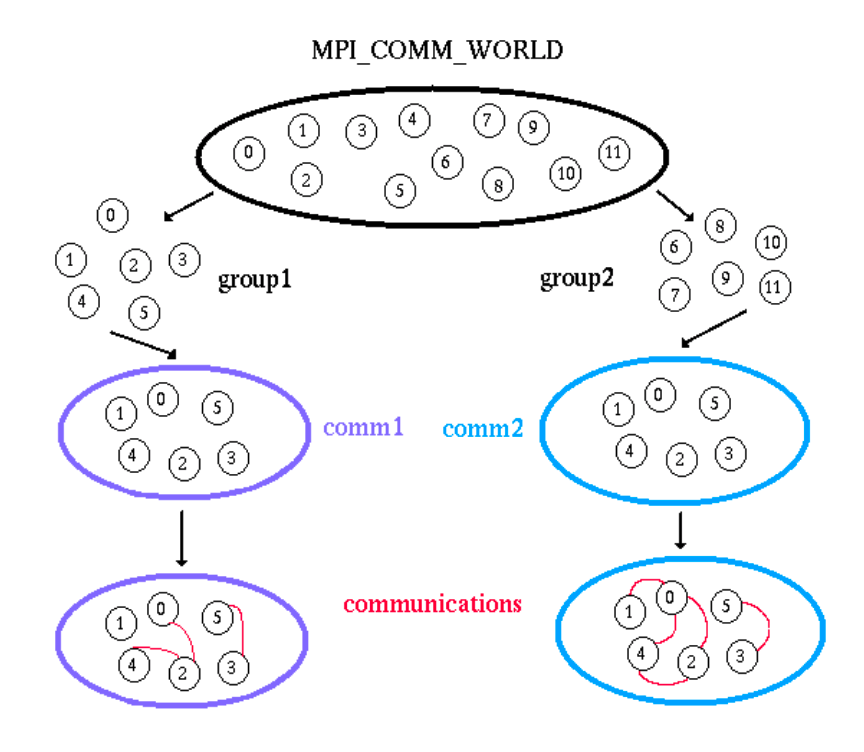
\includegraphics[width=0.7\linewidth]{screenshot027}
\caption{A diagram of groups and communicators.}
\label{fig:screenshot027}
\end{figure}

From  the  programmer's  perspective,  a  group  and  a  communicator  are  one.  The  group routines  are  primarily  used  to  specify  which  processes  should  be  used  to  construct  a communicator.  

The primary purposes of group and communicator objects are:

\begin{itemize}
\item Allow you to organize tasks, based upon function, into task groups.  
\item Enable Collective Communications operations across a subset of related tasks.  
\item Provide basis for implementing user defined virtual topologies  
\item Provide for safe communications  
\end{itemize}

Considerations when using groups and communicators are:
\begin{itemize}
\item Groups/communicators are dynamic - they can be created and destroyed during program execution.  
\item Processes may be in more than one group/communicator. They will have a unique rank within each group/communicator.  
\item MPI provides over 40 routines related to groups, communicators, and virtual topologies.  
\item Typical usage:  \begin{itemize}
  \item Extract handle of global group from \texttt{MPI\_COMM\_WORLD} using \texttt{MPI\_Comm\_group}  
  \item Form new group as a subset of global group using \texttt{MPI\_Group\_incl}  
  \item Create new communicator for new group using \texttt{MPI\_Comm\_create}  
  \item Determine new rank in new communicator using \texttt{MPI\_Comm\_rank}  
  \item Conduct communications using any MPI message passing routine  
  \item When finished, free up new communicator and group (optional) using \texttt{MPI\_Comm\_free} and \texttt{MPI\_Group\_free}  
\end{itemize}
\end{itemize}

MPI includes routines for accessing information on groups or communicators, for creating new groups or communicators from existing ones, and for deleting groups or communicators. 

Communicator creation routines are collective. They require all processes in the input  communicator  to  participate,  and  may  require  communication  amongst processes.  All  other  group  and  communicator  routines  are  local.  It often makes sense to have all members of an input group call a group creation routine, if a communicator will later be created for that group.

\subsection{Group Accessors}
\begin{itemize}
\item\texttt{MPI\_Group\_size} returns number of processes in a group.
\item\texttt{MPI\_Group\_rank} returns rank of calling process in a group.
\item\texttt{MPI\_Group\_translate\_ranks} translates ranks of processes in one group to those in another group.
\item\texttt{MPI\_Group\_compare} compares group members and group order.
\end{itemize}

\subsection{Group Constructors}
\begin{itemize}
\item\texttt{MPI\_Comm\_group} returns the group associated with a communicator.
\item\texttt{MPI\_Group\_union} creates a group by combining two groups.
\item\texttt{MPI\_Group\_intersection} creates a group from the intersection of two groups.
\item\texttt{MPI\_Group\_difference} creates a group from the difference between two groups.
\item\texttt{MPI\_Group\_incl} creates a group from listed members of an existing group.
\item\texttt{MPI\_Group\_excl} creates a group excluding listed members of an existing group.
\item\texttt{MPI\_Group\_range\_incl} creates a group according to first rank, stride, last rank.
\item\texttt{MPI\_Group\_range\_excl} creates a group by deleting according to first rank, stride, last rank.
\end{itemize}

\subsection{Group Destructors}
\begin{itemize}
\item\texttt{MPI\_Group\_free} marks a group for deallocation.
\end{itemize}

\subsection{Communicator Accessors}
\begin{itemize}
\item\texttt{MPI\_Comm\_size} returns number of processes in communicator's group.
\item\texttt{MPI\_Comm\_rank} returns rank of calling process in communicator's group.
\item\texttt{MPI\_Comm\_compare} compares two communicators.
\end{itemize}

\subsection{Communicator Constructors}
\begin{itemize}
\item\texttt{MPI\_Comm\_dup} duplicates a communicator.
\item\texttt{MPI\_Comm\_create} creates a new communicator for a group.
\item\texttt{MPI\_Comm\_split} splits a communicator into multiple, non-overlapping communicators.
\end{itemize}

\subsection{Communicator Destructors}
\begin{itemize}
\item\texttt{MPI\_Comm\_free} marks a communicator for deallocation.
\end{itemize}

\section{Virtual Topologies}
In terms of MPI, a virtual topology describes a mapping/ordering of MPI processes 
into a geometric "shape".  The two main types of topologies supported by MPI are Cartesian (grid) and 
Graph.  

MPI topologies are virtual - there may be no relation between the physical 
structure of the parallel machine and the process topology. Virtual topologies are built upon MPI communicators and groups, and must be "programmed" by the application developer.  

Why use them? Virtual topologies may be useful for applications with specific communication patterns - 
patterns that match an MPI topology structure.  For example, a Cartesian topology might prove convenient for an application that requires 4-way nearest neighbor communications for grid based data.  

Additionally, some hardware architectures may impose penalties for communications between 
successively distant "nodes".  A particular implementation may optimize process mapping based upon the physical characteristics of a given parallel machine.  The mapping of processes into an MPI virtual topology is dependent upon the MPI implementation, and may be totally ignored.